\section{Техническое задание}
\subsection{Основание для разработки}

Полное наименование системы: <<Программная система для визуализации объектов в трёхмерном пространстве>>.

Основанием для разработки является приказ ректора ЮЗГУ от <<17>> апреля 2025 г. №1828-с <<О направлении (допуске) на практику>>.

\subsection{Цель и назначение разработки}

Основной целью преддипломной практики является разработка программной системы (графического движка) для визуализации трёхмерных данных в реальном времени для ООО <<Предприятие ВТИ-Сервис>>.

Посредством разработки данного движка планируется решить ряд технических задач, стоящих перед компанией. Цели разработки можно разделить на две основные группы: технические и практические.

Задачами данной разработки являются:

\begin{enumerate}
    \item Реализация базовых компонентов графического конвейера на основе OpenGL.
    \item Создание кроссплатформенного решения с использованием SDL2.
    \item Разработка системы управления шейдерами и текстурами.
    \item Реализация системы камеры.
    \item Создание базовых геометрических примитивов.
    \item Разработка формата файлов сцены.
    \item Разработка системы загрузки и отображения сцен.
\end{enumerate}

\subsection{Требования к программной системе}

\subsubsection{Требования к интерфейсу пользователя}

Интерфейс пользователя должен быть максимально простым для концентрации на визуализации трёхмерных объектов. Один из вариантов внешнего вида окна программы представлен на рисунке \ref{interface:image}.

\begin{figure}[ht]
\center{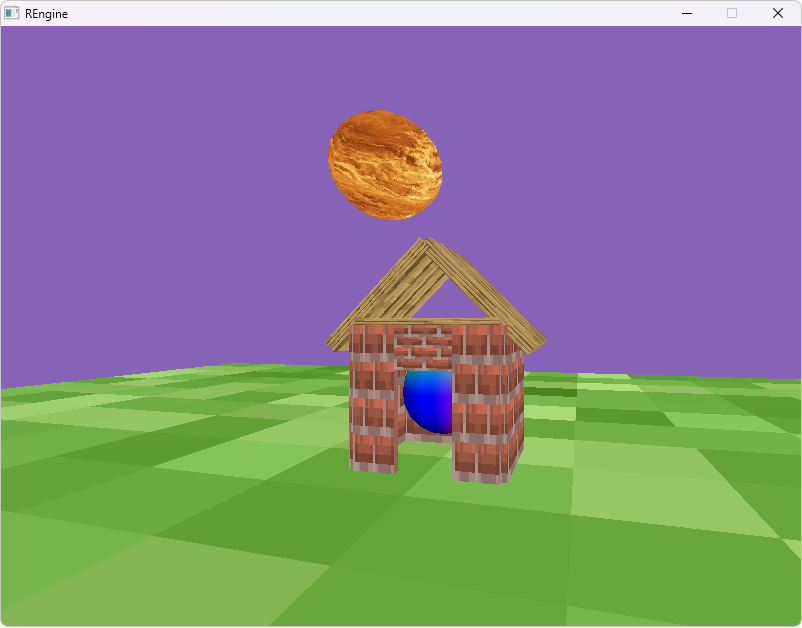
\includegraphics[width=1\linewidth]{screenshot.png}}
\caption{Окно программы}
\label{interface:image}
\end{figure}

\subsubsection{Функциональные требования}

Для разрабатываемого графического движка была построена модель, отражающая основные сценарии его использования в корпоративной среде.

Данная модель помогает выявить ключевые точки интеграции движка с существующими информационными системами предприятия, а также определить роли пользователей и взаимодействие с внешними системами. Для описания сценариев используется унифицированный язык визуального моделирования UML.

Диаграмма вариантов использования описывает функциональное назначение разрабатываемой системы. Она является исходным концептуальным представлением системы в процессе ее проектирования и разработки. Проектируемая система представляется в виде ряда прецедентов, предоставляемых системой актерам или сущностям, которые взаимодействуют с системой. Актером или действующим лицом является сущность, взаимодействующая с системой извне (например, человек, техническое устройство). Прецедент служит для описания набора действий, которые система предоставляет актеру.

На основании анализа предметной области в программе должны быть реализованы следующие прецеденты:

\begin{enumerate}
    \item Отображение заранее созданных трёхмерных сцен с базовыми геометрическими примитивами (кубы, сферы).
    \item Перемещение камеры по трёхмерной сцене с помощью клавиатуры и мыши.
    \item Загрузка и применение текстур к объектам.
    \item Изменение вершинных и фрагментных шейдеров.
    \item Кроссплатформенная работа на операционных системах Windows и Linux.
\end{enumerate}

На рисунке \ref{usecase:image} представлена диаграмма вариантов использования.

\begin{figure}[ht]
\center{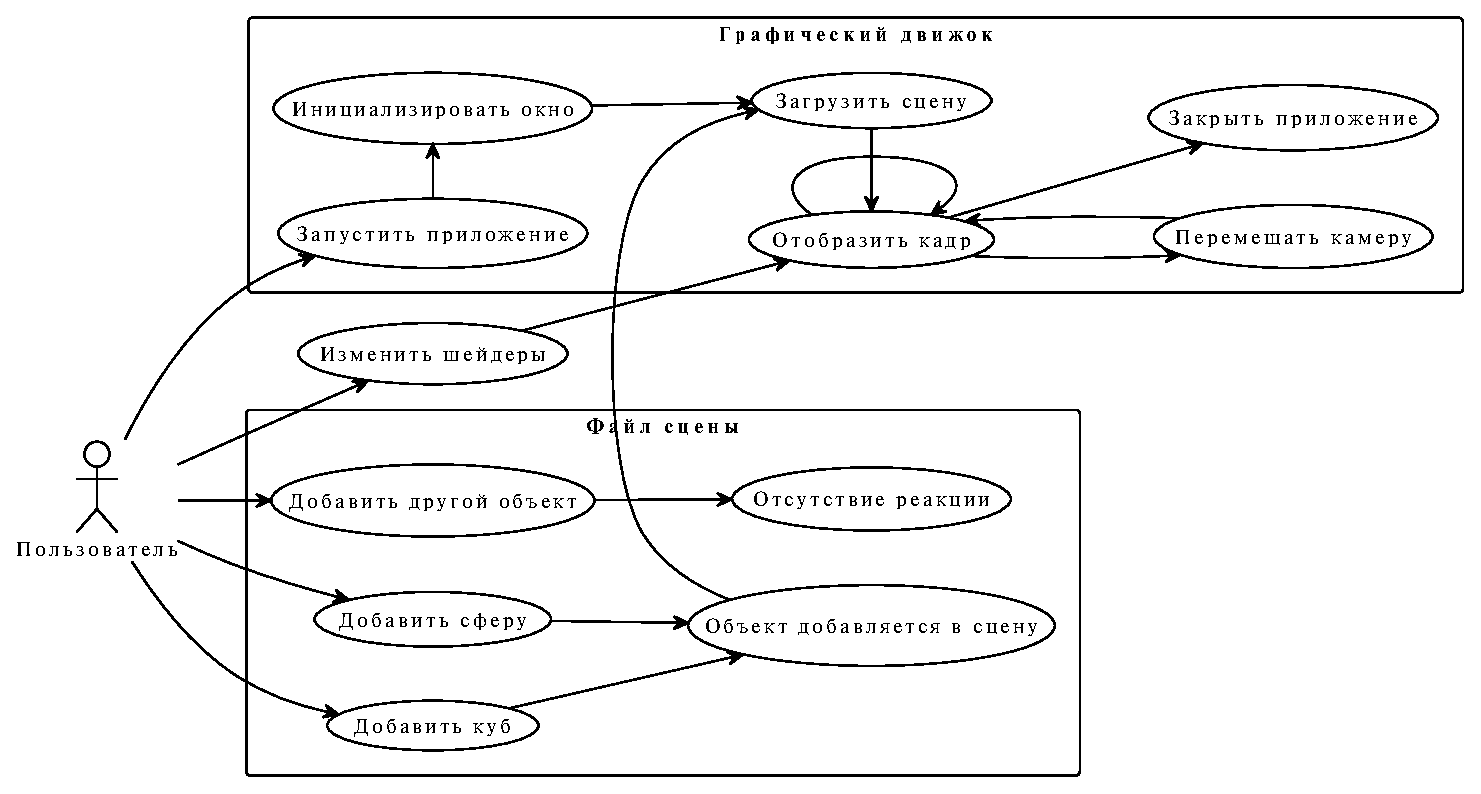
\includegraphics[width=1\linewidth]{usecase}}
\caption{Диаграмма вариантов использования}
\label{usecase:image}
\end{figure}

\paragraph{Вариант использования <<Отображение трёхмерной сцены>>}

Заинтересованные лица и их требования: пользователь желает увидеть трёхмерную сцену. Предусловие: запущена поддерживаемая операционная система, файл сцены присутствует, шейдеры стандартные. Постусловие: пользователь ознакомляется с визуализацией.

\begin{enumerate}
    \item Пользователь запускает приложение.
    \item Приложение инициализирует графический контекст.
    \item Приложение компилирует шейдеры.
    \item Приложение загружает файл сцены.
    \item Приложение создаёт геометрические примитивы.
    \item Приложение отображает трёхмерную сцену.
    \item Пользователь видит трёхмерную сцену.
\end{enumerate}

\paragraph{Вариант использования <<Перемещение камеры>>}

Заинтересованные лица и их требования: пользователь желает перемещать камеру по трёхмерной сцене. Предусловие: запущена поддерживаемая операционная система, файл сцены присутствует, шейдеры стандартные. Постусловие: пользователь имеет возможность увидеть трёхмерную сцену под другим ракурсом.

\begin{enumerate}
    \item Пользователь запускает приложение.
    \item Приложение инициализирует графический контекст.
    \item Приложение компилирует шейдеры.
    \item Приложение загружает файл сцены.
    \item Приложение создаёт геометрические примитивы.
    \item Приложение отображает трёхмерную сцену.
    \item Пользователь нажимает на клавиши клавиатуры и двигает мышью для перемещения камеры в пространстве.
    \item Приложение обрабатывает ввод и изменяет матрицу вида камеры.
    \item Пользователь видит изменение перспективы камеры.
\end{enumerate}

\paragraph{Вариант использования <<Изменение сцены>>}

Заинтересованные лица и их требования: пользователь желает добавить несколько объектов в трёхмерную сцену. Предусловие: запущена поддерживаемая операционная система, файл сцены присутствует, шейдеры стандартные, текстуры существуют. Постусловие: пользователь видит изменённую его руками трёхмерную сцену.

\begin{enumerate}
    \item Пользователь открывает файл сцены.
    \item Пользователь добавляет объект типа <<куб>> в сцену.
    \item Пользователь добавляет объект типа <<сфера>> в сцену.
    \item Пользователь добавляет объект типа <<цилиндр>> в сцену.
    \item Пользователь изменяет начальное положение камеры.
    \item Пользователь добавляет путь к текстуре к созданному объекту <<куб>>.
    \item Пользователь запускает приложение.
    \item Приложение инициализирует графический контекст.
    \item Приложение компилирует шейдеры.
    \item Приложение загружает файл сцены.
    \item Приложение игнорирует объект типа <<цилиндр>>, поскольку он не реализован в программе.
    \item Приложение загружает текстуру по указанному пути и применяет её к объекту <<куб>>.
    \item Приложение создаёт геометрические примитивы.
    \item Приложение отображает трёхмерную сцену.
    \item Пользователь видит трёхмерную сцену.
\end{enumerate}

\paragraph{Вариант использования <<Изменение шейдеров>>}

Заинтересованные лица и их требования: пользователь желает изменить шейдеры, применяемые для отображения объектов в трёхмерной сцене. Предусловие: запущена поддерживаемая операционная система, файл сцены присутствует, шейдеры стандартные. Постусловие: пользователь видит трёхмерную сцену с изменёнными шейдерами.

\begin{enumerate}
    \item Пользователь изменяет вершинный шейдер в соответствии с спецификацией языка GLSL.
    \item Пользователь изменяет фрагментный шейдер в соответствии с спецификацией языка GLSL.
    \item Пользователь запускает приложение.
    \item Приложение инициализирует графический контекст.
    \item Приложение компилирует шейдеры.
    \item Приложение загружает файл сцены.
    \item Приложение создаёт геометрические примитивы.
    \item Приложение отображает трёхмерную сцену.
    \item Пользователь видит трёхмерную сцену с визуальными изменениями, соответствующими изменённым шейдерам.
\end{enumerate}

\subsection{Нефункциональные требования к программной системе}

\subsubsection{Требования к программному обеспечению}

Для реализации разрабатываемого движка должны использоваться языки программирования C++ и GLSL, компилятор GCC и система сборки CMake.

Для запуска и работы с движком требуется использование компьютера под управлением 64-битной операционной системы Windows 7 (или выше) или Linux.

\subsubsection{Требования к аппаратному обеспечению}

Клиентское оборудование должно иметь центральный процессор с частотой ядра не менее 1 ГГц и поддержкой SSE2, а также видеокарту с поддержкой OpenGL 3.3 или выше. Объём оперативной памяти -- 512 ГБ.

Доступ к сети Интернет не требуется.

\subsection{Требования к оформлению документации}

Разработка программной документации и программного изделия должна производиться согласно ГОСТ 19.102-77 и ГОСТ 34.601-90. Единая система программной документации.
